\documentclass{beamer}
\usepackage[latin1]{inputenc}
\usepackage{tikz}
\usepackage{makecell}
\usetheme{Berlin}
\usetikzlibrary{
	arrows.meta,
	chains,
	decorations.pathreplacing,
	automata,
	positioning,
	scopes,
	quotes,
	shapes	
}

\title{Fast Decompression Lucene Codec}
\author{Ivan Mamontov\\ Grid Dynamics}
\institute{Berlin Buzzwords}
\date{Jun 1st, 2015}

\begin{document}
	\begin{frame}
		\titlepage
	\end{frame}
	\begin{frame}
    		\begin{itemize}
    		    \item TOC!!!
		\end{itemize}
  	\end{frame}
  	\begin{frame}
  		\frametitle{Data encoding and file formats}
  		\begin{itemize}
  			\item Lucene 3.x and before
  			\begin{itemize}
  				\item Tuned to pre-defined data types
  				\item Combinations of delta encoding and variable length byte encodings
  				\item Hardcoded choices -- impossible to customize
  				\item Dependencies on specific file-system behaviors
  				\item Data coding happened in many places
  			\end{itemize}
	  			\item Lucene 4 and onwards
  					\begin{itemize}
  						\item All data writing and reading abstracted from data encoding
  						\item Highly customizable, easy to use API
  					\end{itemize}		
  		\end{itemize}
  	\end{frame}
  	\begin{frame}
  		\frametitle{Lucene 5.0 index format}
  		The default Lucene50 codec is:
  		\begin{itemize}
  			\item variable-byte and fixed-width encoding of delta values
  			\item multi-level skip lists
  			\item natural ordering of docIDs
  			\item encodes both term frequencies and positional information
  		\end{itemize}
  	\end{frame}

  	\begin{frame}
  		\frametitle{What is variable-byte encoding?}
%  		\begin{itemize}
%  			\item uses an integral number of bytes to encode a gap
%  			\begin{itemize}
%  				\item the first bit of the byte is a continuation bit. It is set to 1 for the last byte of the encoded gap and to 0 otherwise
%  				\item the last 7 bits of a byte are \textbf{payload} and encode part of the gap
%  			\end{itemize}
%  		\end{itemize}
  		Encode sequence of numbers into variable-length bytes using one status bit per byte indicating whether the current number expands into next byte.
  	\end{frame}
  	\begin{frame}
  		\frametitle{What is variable-byte encoding?}
  		To encode the decimal number 6917:
		\vskip15pt 
  		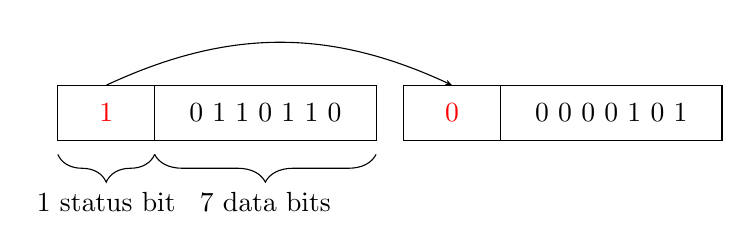
\begin{tikzpicture}[
 		      	start chain = going right,
     			node distance = 0pt,
				ArrayStyle/.style={draw, minimum width=3.5em, minimum 									height=2em, outer sep=0pt, on chain}]
			\node [ArrayStyle] (1) {{\color{red!100}1}};
			\node [ArrayStyle, minimum width=8em] (2) {0 1 1 0 1 1 0};
			\node [ArrayStyle, xshift=1em] (3) {{\color{red!100}0}};
			\node [ArrayStyle, minimum width=8em] (4) {0 0 0 0 1 0 1};
			\begin{scope}[-{Stealth[length = 2.5pt]}]
  				\draw (1.north) [out=25, in=155] to (3.north);
			\end{scope}
			\draw[decorate,decoration={brace, amplitude=10pt, 					raise=5pt, mirror}]
  				(2.south west) to node[black,midway,below= 15pt] 				{$7$ data bits} (2.south east);
			\draw[decorate,decoration={brace, amplitude=10pt, 					raise=5pt, mirror}]
  				(1.south west) to node[black,midway,below= 15pt] 				{$1$ status bit} (1.south east);
		\end{tikzpicture} 
		\vskip15pt 	
		\pause
		Thus needs 2 bytes instead of 4 bytes!
  	\end{frame}
  	\begin{frame}
  		\frametitle{What is variable-byte encoding?}
  		\begin{itemize}
    		    \item pros
    		    \begin{itemize}
    		    		\item wonderfully simple
    		    		\item good compression rate
    		    \end{itemize}
    		    \item cons
    		    \begin{itemize}
    		    		\item it requires an if statement on every byte	during decode, which is very costly since the CPU cannot easily predict the branch outcome.
    		    \end{itemize}
		\end{itemize}
  	\end{frame}
  	\begin{frame}
  		\frametitle{What is PForDelta encoding?}
  		PForDelta -- patched frame-of-reference encoding
  		\begin{itemize}
  			\item takes each fixed block of ints and stores them all as packed ints, where each value gets N bits, set by the maximum int in the block.
  			\item marks large numbers as exceptions, which are then "patched" after the initial decode.	
  		\end{itemize}
  	\end{frame}
  	\begin{frame}
  		\frametitle{What is PForDelta encoding?}
  		To encode the following numbers 1, 3, 7, 10, 13, 14, 18:
		\vskip15pt 
  		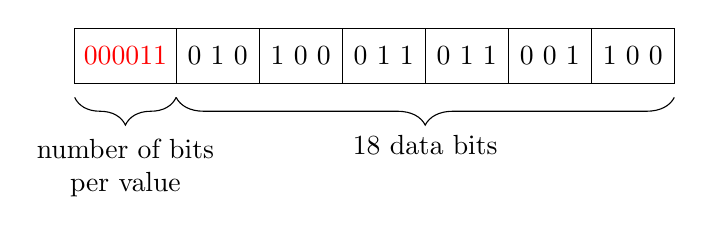
\begin{tikzpicture}[
 		      	start chain = going right,
     			node distance = 0pt,
				ArrayStyle/.style={draw, minimum width=3.5em, minimum 									height=2em, outer sep=0pt, on chain}]		
			\node [ArrayStyle] (1) {{\color{red!100}000011}};
			\node [ArrayStyle, minimum width=3em] (2) {0 1 0};
			\node [ArrayStyle, minimum width=3em] (3) {1 0 0};
			\node [ArrayStyle, minimum width=3em] (4) {0 1 1};
			\node [ArrayStyle, minimum width=3em] (5) {0 1 1};	
			\node [ArrayStyle, minimum width=3em] (6) {0 0 1};
			\node [ArrayStyle, minimum width=3em] (7) {1 0 0};	
			\draw[decorate,decoration={brace, amplitude=10pt, 					raise=5pt, mirror}]
  				(2.south west) to node[black,midway,below= 15pt] 				{18 data bits} (7.south east);
			\draw[decorate,decoration={brace, amplitude=10pt, 					raise=5pt, mirror}]
  				(1.south west) to node[black,midway,below= 15pt] 				{\makecell[c]{number of bits\\per value}} (1.south east);
		\end{tikzpicture} 
		\vskip15pt 	
		\pause
		Thus needs 3 bytes instead of $7*4=32$ bytes!
  	\end{frame}
  	\begin{frame}
  		\frametitle{What is PForDelta encoding?}
  		\begin{itemize}
    		    \item pros
    		    \begin{itemize}
    		    		\item \mbox{ultra-fast} decoding speed.% Up to 2 times faster than in \mbox{variable-byte} encoding
    		    		\item {\color{red!100} TODO something about SIMD/modern CPUs}
    		    \end{itemize}
    		    \item cons
    		    \begin{itemize}
    		    		\item in order to access even one int within the block, we must decode the full block
    		    		\item requires integers in batches of multiples of 32
    		    \end{itemize}
		\end{itemize}  		
  	\end{frame}
  	\begin{frame}
%With conventional scalar operations, four add instructions must be executed one after another to obtain the sums as shown
    		\frametitle{What is SISD?}
    		\begin{itemize}
    		    \item Single Instruction Single Data (SISD)
    		    	\vskip15pt 
    		    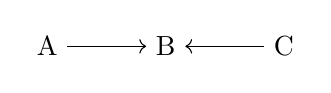
\begin{tikzpicture}[start chain = going right]
   				\node[on chain] (A) {A};
   				\node[on chain,join=by {->}] (B) {B};
   				\node[on chain,join=by {<-}] (C) {C};
			\end{tikzpicture}
		\end{itemize}
  	\end{frame}
  	\begin{frame}
    		\frametitle{What is SIMD?}
    		\begin{itemize}
    		    \item Single Instruction Multiple Data (SIMD)
		    
		\end{itemize}
  	\end{frame}
  	\begin{frame}
    		\frametitle{Why does it matter?}
    		\begin{itemize}
    		    \item pros
    		    \begin{itemize}
    		    		\item 75\% fewer loads
    		    		\item 75\% fewer adds
    		    		\item 75\% fewer stores
    		    \end{itemize}
    		    \item cons
    		    \begin{itemize}
    		    		\item not all algorithms can be vectorized
    		    		\item most compilers don't generate SIMD instructions
    		    		\item SIMD may have restrictions on data alignment
    		    \end{itemize}
		\end{itemize}
  	\end{frame}  	
  	\begin{frame}
  		\frametitle{SIMD auto-vectorization in HotSpot}
  		%Sometimes it is possible to move the kernel to C/C++, use SIMD there and call via JNI. However, the cost of the JNI call can be significant as are the difficulties of ensuring memory is properly aligned for SIMD execution
  		%In HotSpot versions beginning with Java 7u40, the server compiler provides support for auto-vectorisation. According to JDK-6340864
		%However, this seems to be true only for "simple loops" - at least for the moment. For example, accumulating an array cannot be vectorised yet JDK-7192383
		Vector arithmetic is not supported yet. Only array initialization and array copy.
  		\begin{itemize}
  			\item \url{http://bugs.java.com/view_bug.do?bug_id=6340864}
  			\item \url{http://bugs.java.com/view_bug.do?bug_id=7192383}
  		\end{itemize}
  	\end{frame}
  	\begin{frame}
  		\frametitle{Cost of JNI Call	in HotSpot}
  	\end{frame}
\end{document}